\subsection{B\"{u}chi Automaton Pruning}
\label{subsubsec:NBA-pruning}
As the first step, the NBA~$\mathcal{B}_{\varphi}$ associated with the task~$\varphi$
is derived, e.g., via translation tools~\cite{gastin2001fast}.
Note that~$\mathcal{B}_{\varphi}$ has the structure as defined in Def.~\ref{def:nba},
which however can be overly redundant.
For instance, the required input alphabets for some transitions are infeasible for the whole team;
or some transitions are redundant as they can be decomposed equivalently
into other transitions.
Via detecting and removing such transitions, the size of the underlying NBA
can be greatly reduced, thus improving the efficiency of subsequent steps.
More specifically, pruning of~$\mathcal{B}_{\varphi}$ consists of the following three steps:

(i) Remove infeasible transitions.
Given any transition $q_j \in \delta(q_i,\, \sigma)$ in~$\mathcal{B}_{\varphi}$,
it is infeasible for the considered system if
no subgroup of agents in~$\mathcal{N}$ can generate $\sigma$.
It can be easily verified by checking whether there exist an agent that can navigate to region~$W_m$ and perform local action~$a_k$;
or several agents that can \emph{all} navigate to region~$W_m$ and perform collaborative action~$a_k$.
If infeasible, such transition is removed in the pruned automaton.

(ii) Remove invalid states.
Any state~$q\in Q$ in~$\mathcal{B}_{\varphi}$ is called invalid
if it can not be reached from any initial state;
or it can not reach any accepting state that is in turn reachable from itself.
An invalid state can not be part of an accepting path thus removed in the pruned automaton.

(iii) Remove decomposable transitions.
Due to the distributed nature of multi-agent systems,
it is unrealistic to enforce the fulfillment of two or more subtasks
to be \emph{exactly} at the same instant in real time.
Therefore, if possible,
any transition that requires the simultaneous satisfaction of several sub-tasks is decomposed into equivalent transitions.
Decomposable transitions are formally defined in
Def.~\ref{def:decomposable-transition} below.
In other words, the input alphabets of a decomposed transition can be mapped to
two other transitions that connect the \emph{same} pair of states,
but via another intermediate state, as illustrated in Fig.~\ref{fig:example_decomposable}.
Thus, all decomposable transitions in~$\mathcal{B}_{\varphi}$ are removed in the pruned automaton.
Algorithmically, decomposability can be checked by simply composing and comparing the
propositional formulas associated with each transition.

\begin{definition}[Decomposable Transition]\label{def:decomposable-transition}
Any transition from state~$q_i$ to $q_j$ in~$\mathcal{B}_{\varphi}$ is decomposable if there exists another state $q_k$ such that $q_j\in \delta(q_i,\sigma_{ik}\cup\sigma_{kj})$ holds,
$\forall \sigma_{ik},\,\sigma_{kj} \subseteq \Sigma$ that $q_k\in \delta(q_i,\sigma_{ik})$ and $q_j\in \delta(q_k,\sigma_{kj})$ hold.
\hfill $\blacksquare$
\end{definition}

An example of decomposable transitions is shown in Fig.~\ref{fig:example_decomposable}.
To summarize, the pruned NBA, denoted by~$\mathcal{B}^{-}_{\varphi}$,
has the same structure as~$\mathcal{B}_{\varphi}$ but with much fewer states and edges.
In our experience, this pruning step can reduce up to $60\%$ states and edges for typical multi-agent tasks.
More details can be found in the experiment section. 
\begin{lemma}
  If there exists a word~$\omega$ that is accepted by~$\mathcal{B}$,
  then an equivalent run~$\omega'$ can be found that is accepted by~$\mathcal{B}^-$.
\end{lemma}
\begin{proof}
  Consider an accepting word $\omega=\cdots\{\sigma_1\land\sigma_2\}\cdots$
  and the associated run in~$\mathcal{B}$ is given by~$\rho=\cdots q_1 q_3\cdots$ of $\mathcal{B}$.
  Thus there exists state~$q_2$ satisfying that 
  $q_2=\delta(\sigma_1,q_1)$, $q_3=\delta(\sigma_2,q_2)$, $q_3=\delta(\sigma_1\land\sigma_2,q_1)$.
  Moreover, as the labels are not instantaneous, 
  an equivalent \emph{word} $\omega'=\cdots\{\sigma_1\land\sigma_2\}\{\sigma_1\land\sigma_2\}\cdots$
  can be created by adding an additional time step.
  The associated run in~$\mathcal{B}^-$ is given by~$\rho'=\cdots q_1 q_2 q_3\cdots$ where
  $q_2=\delta(\sigma_1\land\sigma_2,q_1)$, $q_3=\delta(\sigma_1\land\sigma_2,q_2)$.
  This completes the proof.
\end{proof}
%=================================




%========================================


\begin{figure}
\centering
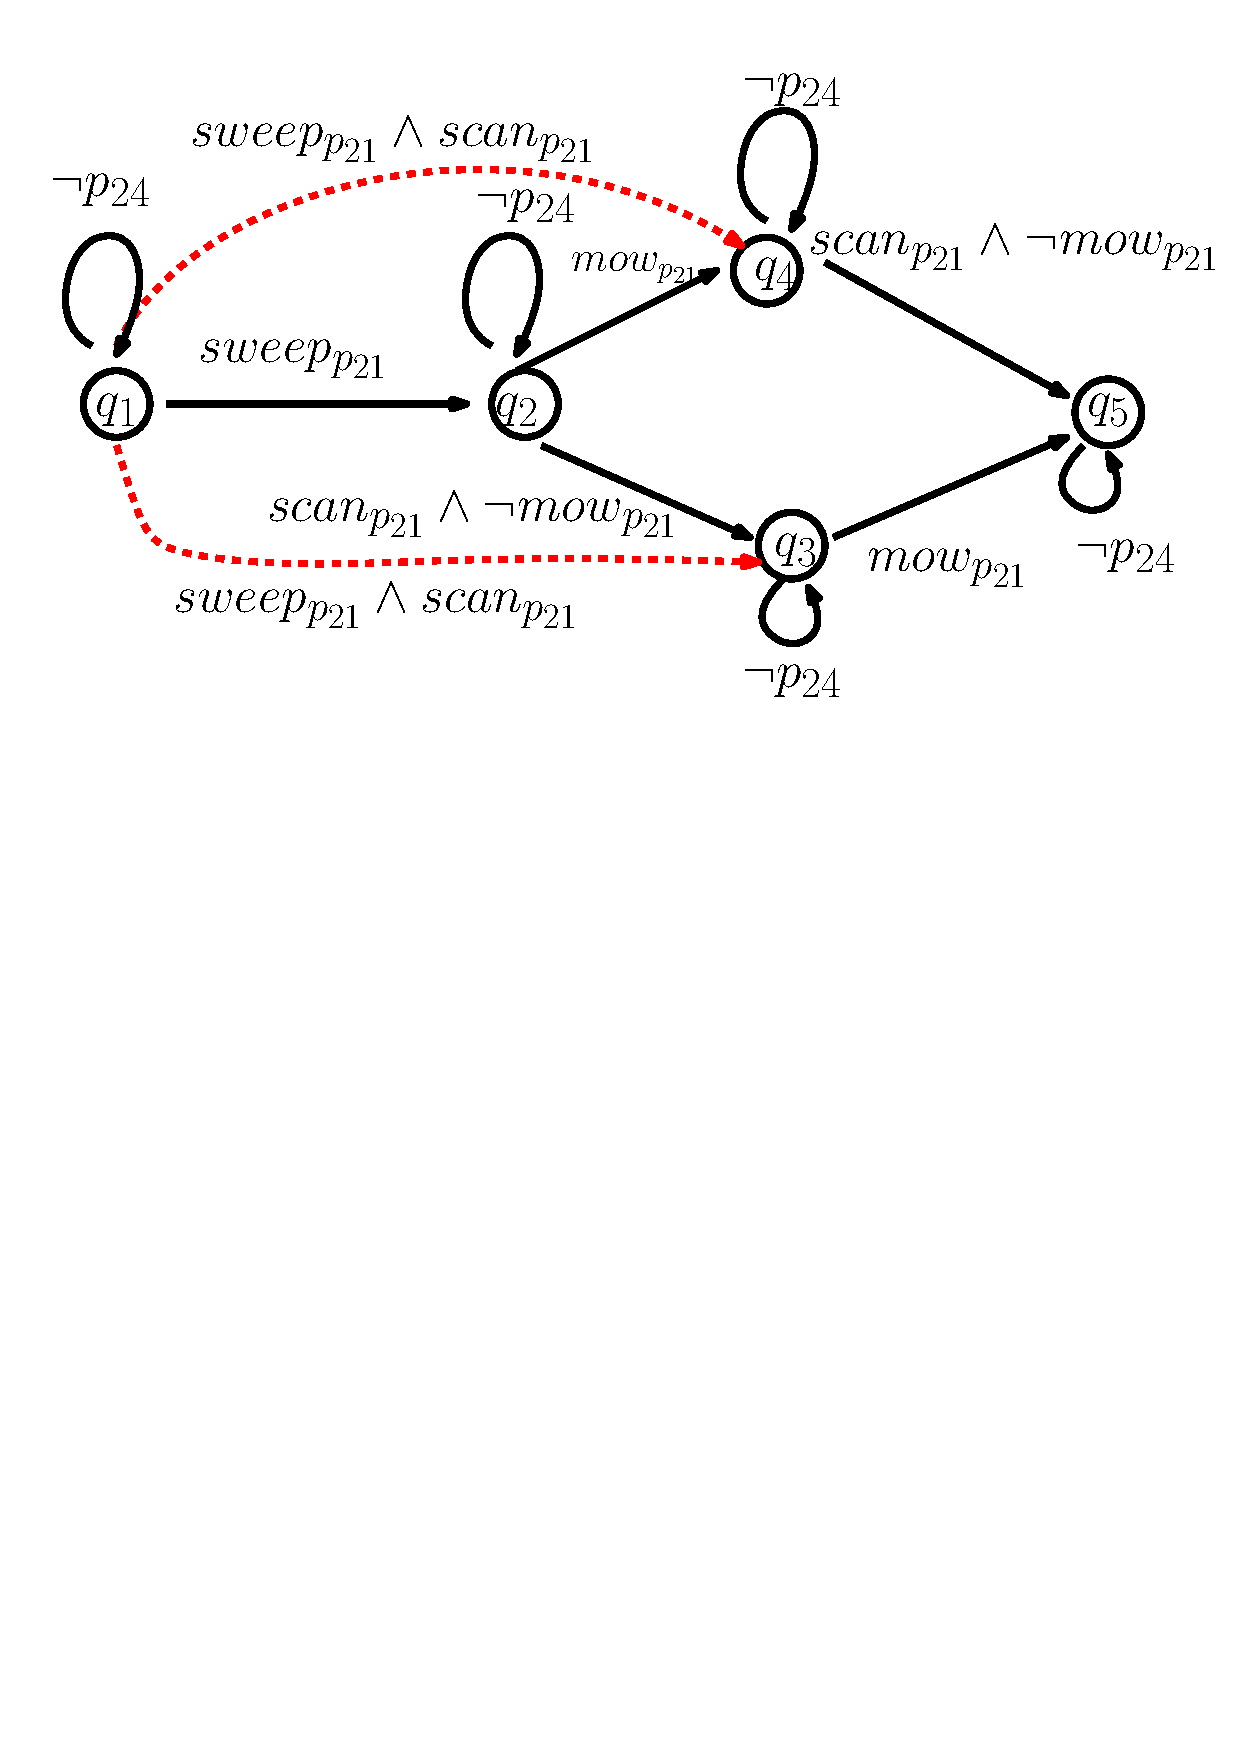
\includegraphics[scale=0.4]{figures/example_decomposable.pdf}
\caption{
Example of decomposable transitions.
Any transition in red dashed line are all 
decomposable satisfied by Def.~\ref{def:decomposable-transition}.}
\label{fig:example_decomposable}
\end{figure}
%========================================

\begin{example}\label{eq:prune-nba}
The NBA~$\mathcal{B}_{\varphi}$ associated with the task formula in~\eqref{example:task}
has $707$ states and $16044$ edges with more than $1.29\times10^7$ accepting \emph{word},
translated via~\cite{gastin2001fast}.
After the pruning process described above, the pruned automaton~$\mathcal{B}^{-}_{\varphi}$
has $707$ states and $2423$ edges with $174469$ accepting \emph{word}. The NBA pruning step reduces $84.9\%$ edges and $98.6\%$
accepting \emph{word} without losing any information.
\hfill $\blacksquare$
\end{example}
